\documentclass{article}
\usepackage{amsmath, amssymb, cite, algorithmic, url, braket}
\usepackage{graphicx}
\usepackage{pythonhighlight}
\usepackage[margin=1.5cm]{geometry}
\usepackage[title]{appendix}
\usepackage{subfigure}
\usepackage{listings}
\usepackage{booktabs}

\graphicspath{{../pic/}}
\lstset{
language=[ANSI]{C},
showtabs=true,
tab=,
tabsize=2,
basicstyle=\ttfamily\footnotesize,%\setstretch{.5},
stringstyle=\color{stringcolour},
showstringspaces=false,
alsoletter={1234567890},
otherkeywords={\%, \}, \{, \&, \|},
keywordstyle=\color{keywordcolour}\bfseries,
upquote=true,
morecomment=[s]{/*}{*/},
commentstyle=\color{commentcolour}\slshape,
literate=*%
{=}{{\literatecolour=}}{1}%
{-}{{\literatecolour-}}{1}%
{+}{{\literatecolour+}}{1}%
{*}{{\literatecolour*}}{1}%
{!}{{\literatecolour!}}{1}%
{[}{{\literatecolour[}}{1}%
{]}{{\literatecolour]}}{1}%
{<}{{\literatecolour<}}{1}%
{>}{{\literatecolour>}}{1}%
% {>>>}{\pythonprompt}{3}%
,%
frame=trbl,
rulecolor=\color{black!40},
backgroundcolor=\color{white},
breakindent=.5\textwidth,frame=single,breaklines=true
}

\begin{document}
\title{DSP Homework 07}
\author{Xu, Minhuan}
\maketitle
\tableofcontents
\begin{abstract}
\subsubsection*{Videos}
After summing up the videos, I find out the maximum of speed of my mouse.
\subsubsection*{Pros and Cons of Shannon/Nyquist sampling method}
I will explain what and why the Shannon/Nyquist sampling method is good and also bad.
\subsubsection*{Trajectory of My Phone}
Using a cutting board as the background of the video, I draw the trajectory of my phone by a method which is similar with IAS in mice.
\end{abstract}

\section{Videos}
\subsection{Image Processing in Mice}
There are a lot of parts which cooperate with each other, but in this video we mainly know about things about image processing unit which is called Image Acquisition System (IAS) and interpolation.

\subsubsection{IAS}

The IAS contains a infrared LED, a pair of lenses, and the image pixel array. 

About the LED, we can't see the infrared ray with our eyes, but many years ago we do see some light came out from the bottom of our mice.

And the pair of lenses, one is to refract the ray in order to let the ray hits the surface in a very small angle, the other is to receive the reflected ray. About the reflected ray, since it is shot on the rough surface in a small angle, so the high part of the surface will block the light which would hit the lower place if the surface was flat. So we can simply consider the higher place will be bright, and the lower place will be rather dim.

The last part is the image pixel array. This can be called a image sensor by itself. It can translate the light and the shade into a black and white picture. This picture won't be stored in the mouse, but be compared with the picture transmitted into the image sensor. So, how do the mouse know the displacement in $x$ and $y$?

It turns out that in the mouse there's a DSP chip which keep calculating the cross correlation of previous and present picture shot by the image sensor. If found the cross correlation is not large enough, which means the mouse has made a move, the processor will move the image in $x-y$ plane and calculate the cross correlation again. The processor will keep do that until there's a maximum of the value of cross correlation, then, only the corresponding displacement of the maximum is what the processor cares. The IAS usually takes $17,000$ pictures of the surface every second, and this means that the processor will compares the present picture to the previous picture every $59 ~\mathrm{\mu s}$. But the chip in mice will only reports to the computer every $1 ~\mathrm{\mu s}$.

\subsubsection{Interpolation}
In the level of hardware, some mice have image sensors with $40 \times 40$ pixels. So, the raw data from that sensor will be $1,600$ digits which range in $0 \sim 4095$ and represent the intensity of light. But we can still use interpolation to get more useful digits. That means apart from real points \emph{see} by the sensor, the chips in the mice will \emph{imagine} more points. The value of those \emph{imagined} points are determined by the real points around.

\subsection{Starch-Based Diets make us healthy}
The lecturer is a doctor who has been searching for the way of making people healthy for over 40 years. He want to convince us that it is good for human to have starch-based diets in three aspects as below:

\begin{enumerate}
	\item Throughout human history, bulk of people have had the starch-based diets.
	\item People who from the areas in which people have the habit of living on starch have less sickness even though they has moved to meat-eating areas.
	\item Children, military, workers, and many other people in the USA are getting overweight and sick.
\end{enumerate}

\subsection{Our Planet}
This episode of Our Planet is about the creatures in the polar regions.

In Antarctica, krill is eaten by Gentoo Penguins and humpback whales, Gentoo Penguins are eaten by killer whales. However, with warming temperatures and disappearing sea ice, krill which depend on the sea ice algae have been getting less and less.

In island of South Georgia, the camera tells us that how difficult it is for the king penguins to reach the nursery of their from the sea. There are leopard seals who want to eat them, elephant seals who will flatten them and others' chicks who are mixed with their own chicks.

In Arctic, polar bears and seals suffer from the loss of ice. Moreover, the walrus who once live on the ice, will occupy every square centimeters just to lie down on a tiny island. Some of the even climb onto a hill and drop from that place.

For thousands of years, there's been a balance in the advance and retreat of the sea ice, but that is no longer the case. All we can know from these scenes, many are starting to lose the place where they rest, breed, hunting.

\subsection{Further Thoughts}
Since the mice judge the displacement through the image, so I wonder if I move a mouse so fast that a picture transmitted into the chips is total different from the previous one, it will be lost and make mistake. So I want to calculate how fast can the mouse be lost. But since I cannot make my mouse move so fast, I don't want to implement this experiment.

First, from the video I know that every $\mu\mathrm{s}$ the sensor will take a picture of the surface and report it every $59 ~ \mu\mathrm{s}$, so I think the during time here will be $59 ~ \mu \mathrm{s}$. 

Second, the length of my mouse's lens is about $1 \sim 4 ~ \mathrm{mm}$, so the speed of my mouse must beyond:
$$
v = \frac{x}{t} = \frac{1 \times 10^{-3}}{6 \times 10^{-5}} \approx 16.6 ~\mathrm{m/s}
$$
to let my mouse to be lost.

Finally, I referred the data on the official website and found that the official value of the maximum of speed is about $10.2 ~\mathrm{m/s}$, and that's close.

\section{Pros and Cons of Shannon/Nyquist sampling method}
\subsection{Positive}
\subsubsection{Ideal and easy to understand}
In Shannon/Nyquist sampling method, we only consider things that are ideal. Like $\delta(t)$, and the ideal LPF. It is mathematically simple and friendly to beginners.
\subsubsection{Easy to calculate}
Using Fourier series and Fourier transform, we can easily find the distribution of energy on the frequency domain since the $\delta$ function has nice special properties.

\subsubsection{No Error}
Through calculation, we know that if we make $f_s$ and $f_c$ have proper values, a perfectly the same frequency spectrum can be reconstructed. This is good because we don't need to worry about making mistake through communication.

\subsubsection{Easy to Reconstruct}
Assuming that we have a sampled signal, all we should do is to find the bandwidth, and to let the sampled signal pass a LPF. Then, a perfectly reconstructed signal is complete.

\subsection{Negative}
\subsubsection{Non-existent signal}
Though the sampling progress is theoretically easy to carry out, the $\delta$ function is not so easy to generate. Mathematically, it has infinite energy in \emph{one} period. According to the law of conservation of energy, we can't make a signal like the $\delta(t)$, see (\ref{eq:energyOfPulse}).
\begin{equation}
E = \sum_{n = -\infty}^{\infty} T \to \infty
\label{eq:energyOfPulse}
\end{equation}

\subsubsection{Waste of bandwidth}
In practical usage, engineers cannot find a ideal LPF, especially which has infinite differential (has a sharp drop). All we can find is those which have smooth differential, and LPF like these will occupy more bandwidth of channels. Then, because

$$
f_c < f_s - W
$$

Therefore, the sampling frequency $f_s$ need to be larger which is not good.

\section{The Trajectory of My Phone}

\subsection{Implement}
Since the Image Acquisition System in mice determine the displacement through the relative $x-y$ coordinates, what I need first is an axis. So I find out a cutting board, see Fig.~\ref{fig:cuttingBoard}

\begin{figure}[!h]
	\centering
	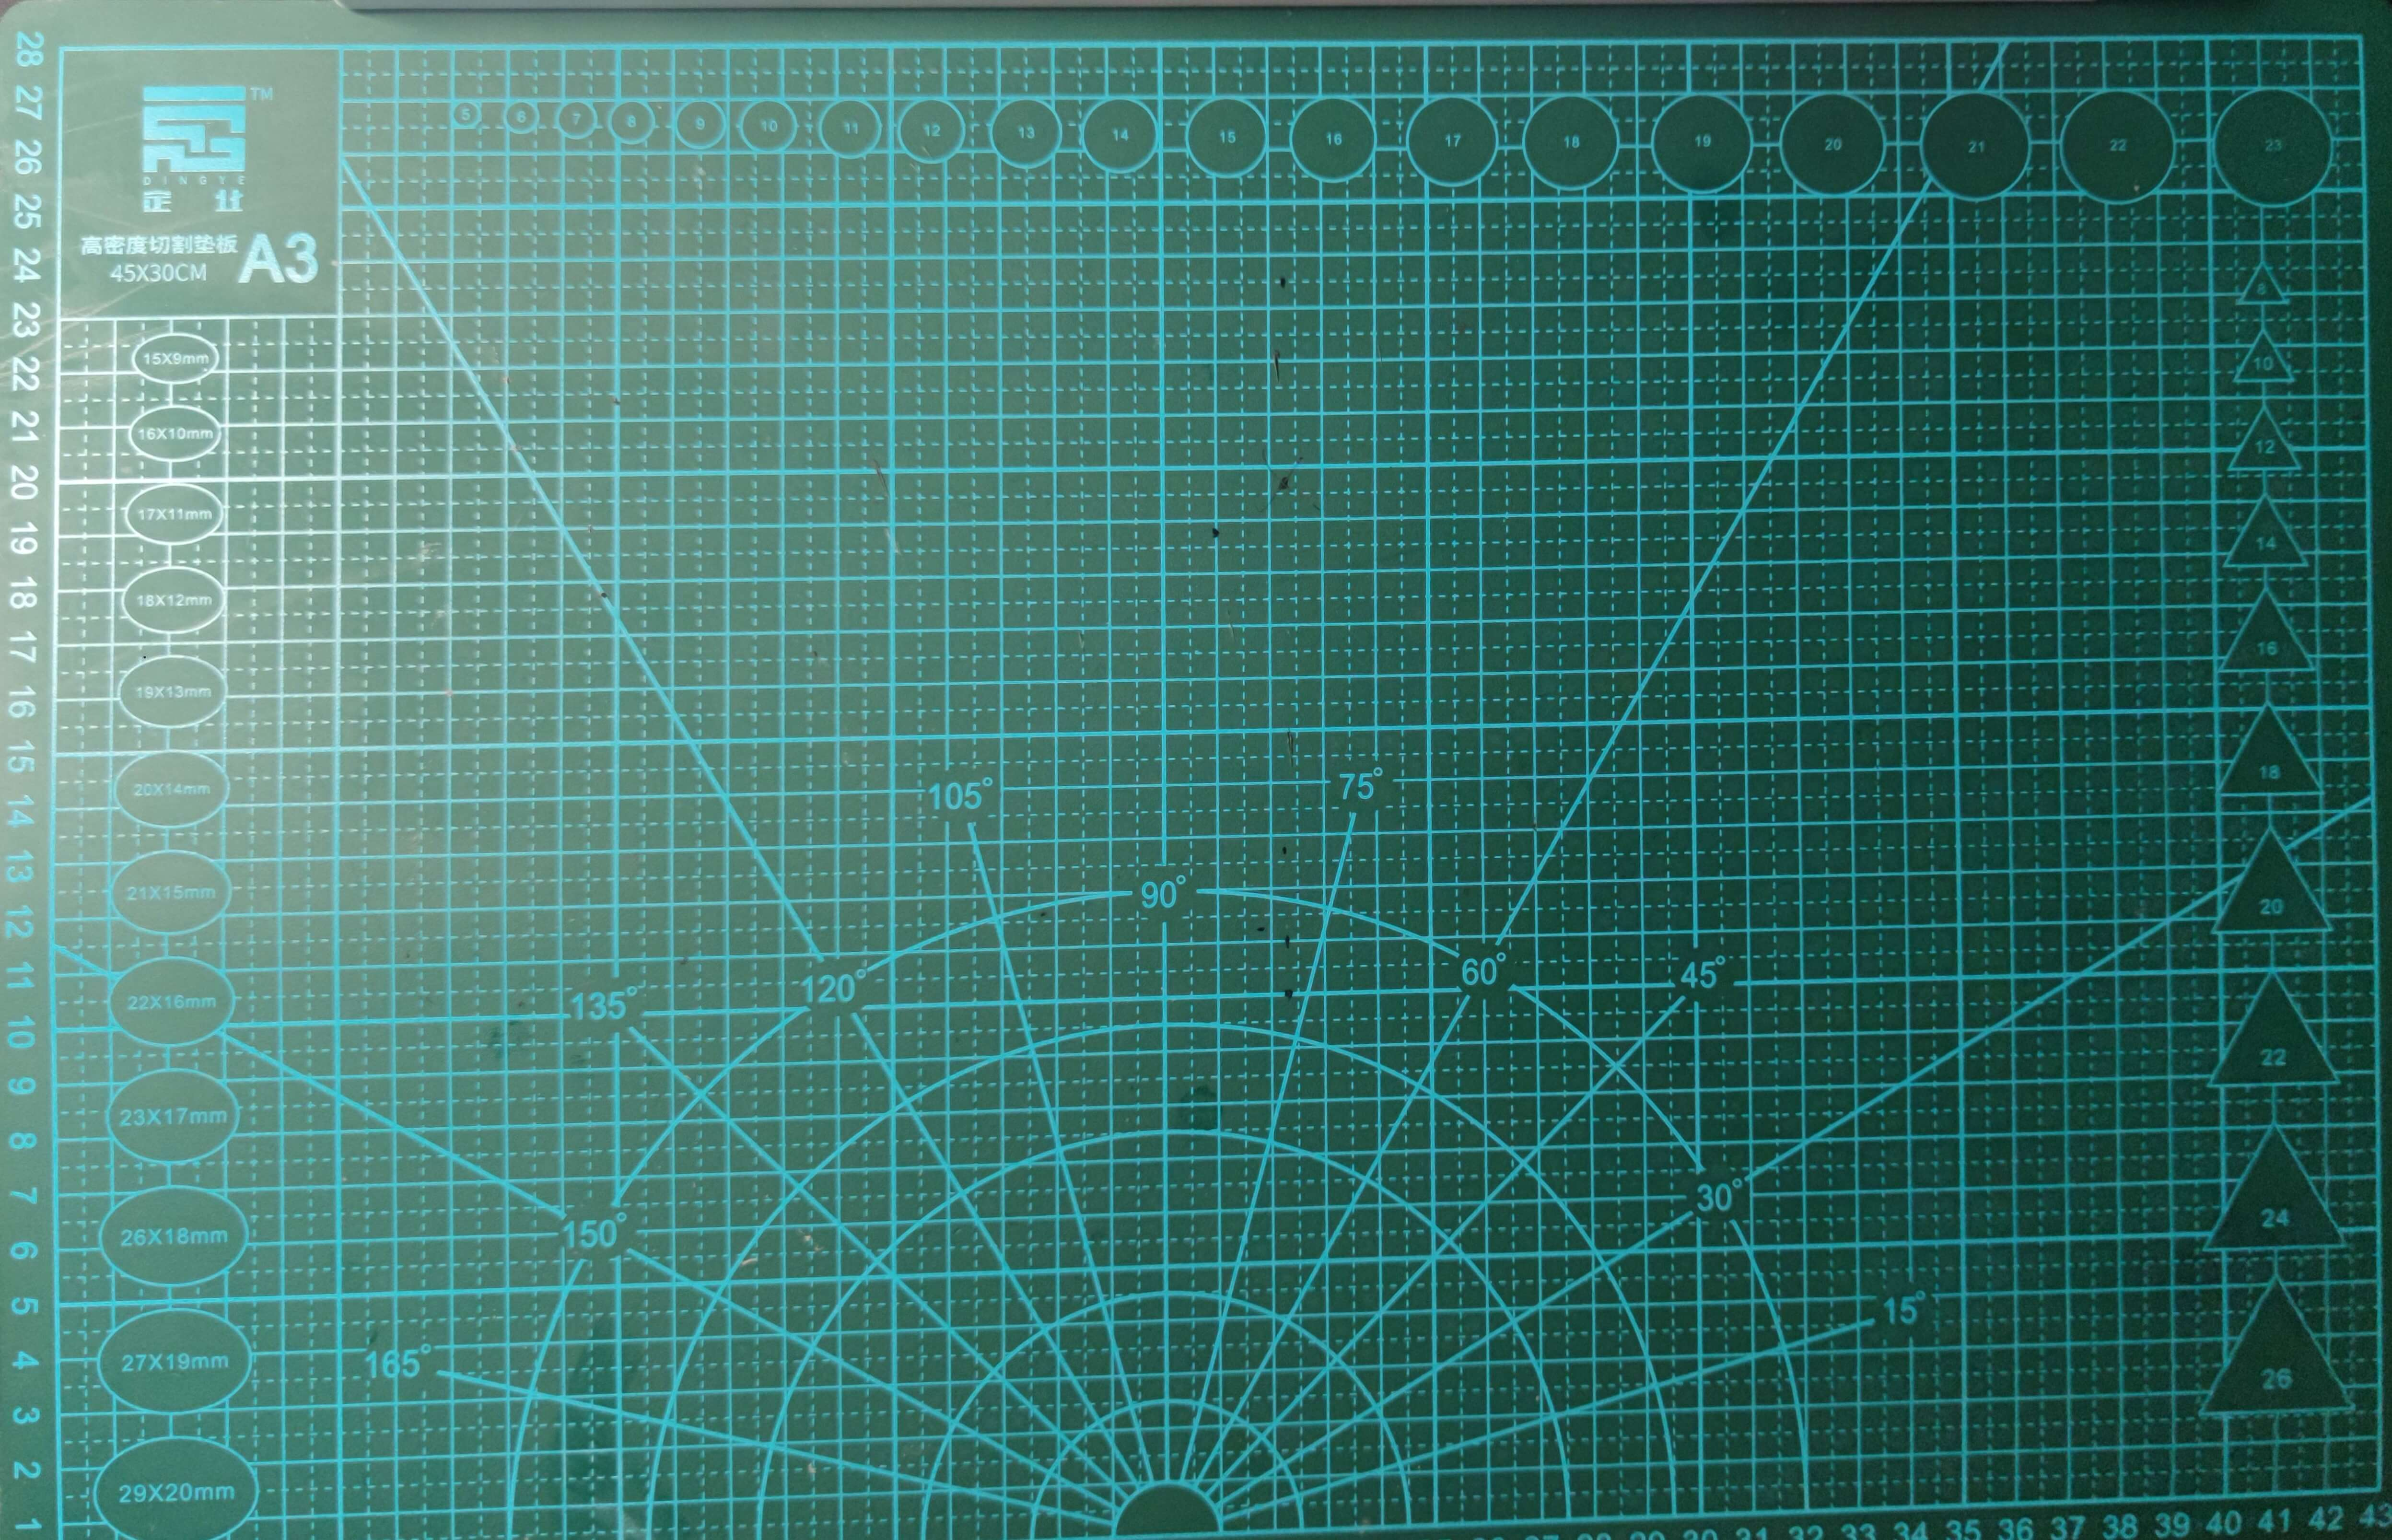
\includegraphics[width=3 in]{../pic/cuttingBoard.jpg}
	\caption{My Cutting Board}
	\label{fig:cuttingBoard}
\end{figure}

\subsubsection{Horizontal}
So I use this board as my background of the video. Next I want to specify how I can know the shift in $x, y, z$. First, for $x, y$, I want to use the middle point in the video as the place where my phone is, and compare the present frame and the previous frame in order to decide the displacement horizontally. 

\subsubsection{Vertical}

Vertically, I take inspiration from similar triangular pyramid in which the area of the bottom is proportional to the height (see Fig.~\ref{fig:blocksAndPyramid}(a)), so I decide to use the square root of the number of blocks in one cut (represents the area of the bottom), which means when the there's 16 blocks in one frame, the \emph{height} will be $4$ \emph{height units} (referred as hu) in my estimation. Another example please see Fig.~\ref{fig:blocksAndPyramid}(b). 

Afterwards, I measured that when my phone was at the height of $10~ \mathrm{cm}$, the $z$ was about $8.5 \mathrm~{hu}$ in my theory. So I will draw my trajectory of my phone using centimeters rather than the hu which is defined by me.  

\begin{figure}[!h]
	\centering
	\subfigure[Triangular Pyramid]{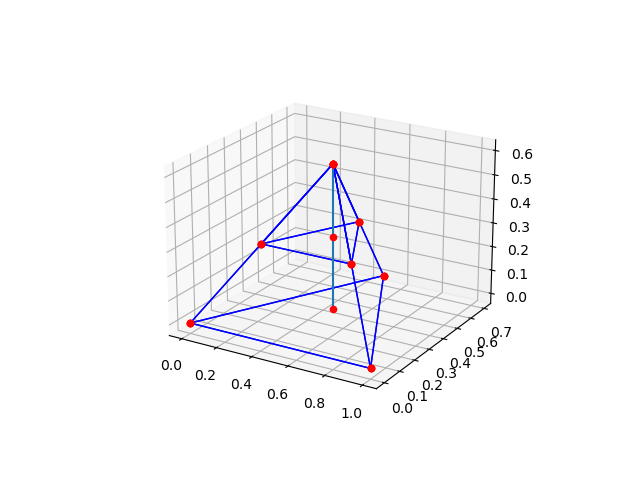
\includegraphics[height=3 in]{../pic/tri-pyramid.png}}
	\hspace{0 pt}
	\subfigure[Blocks in One Frame]{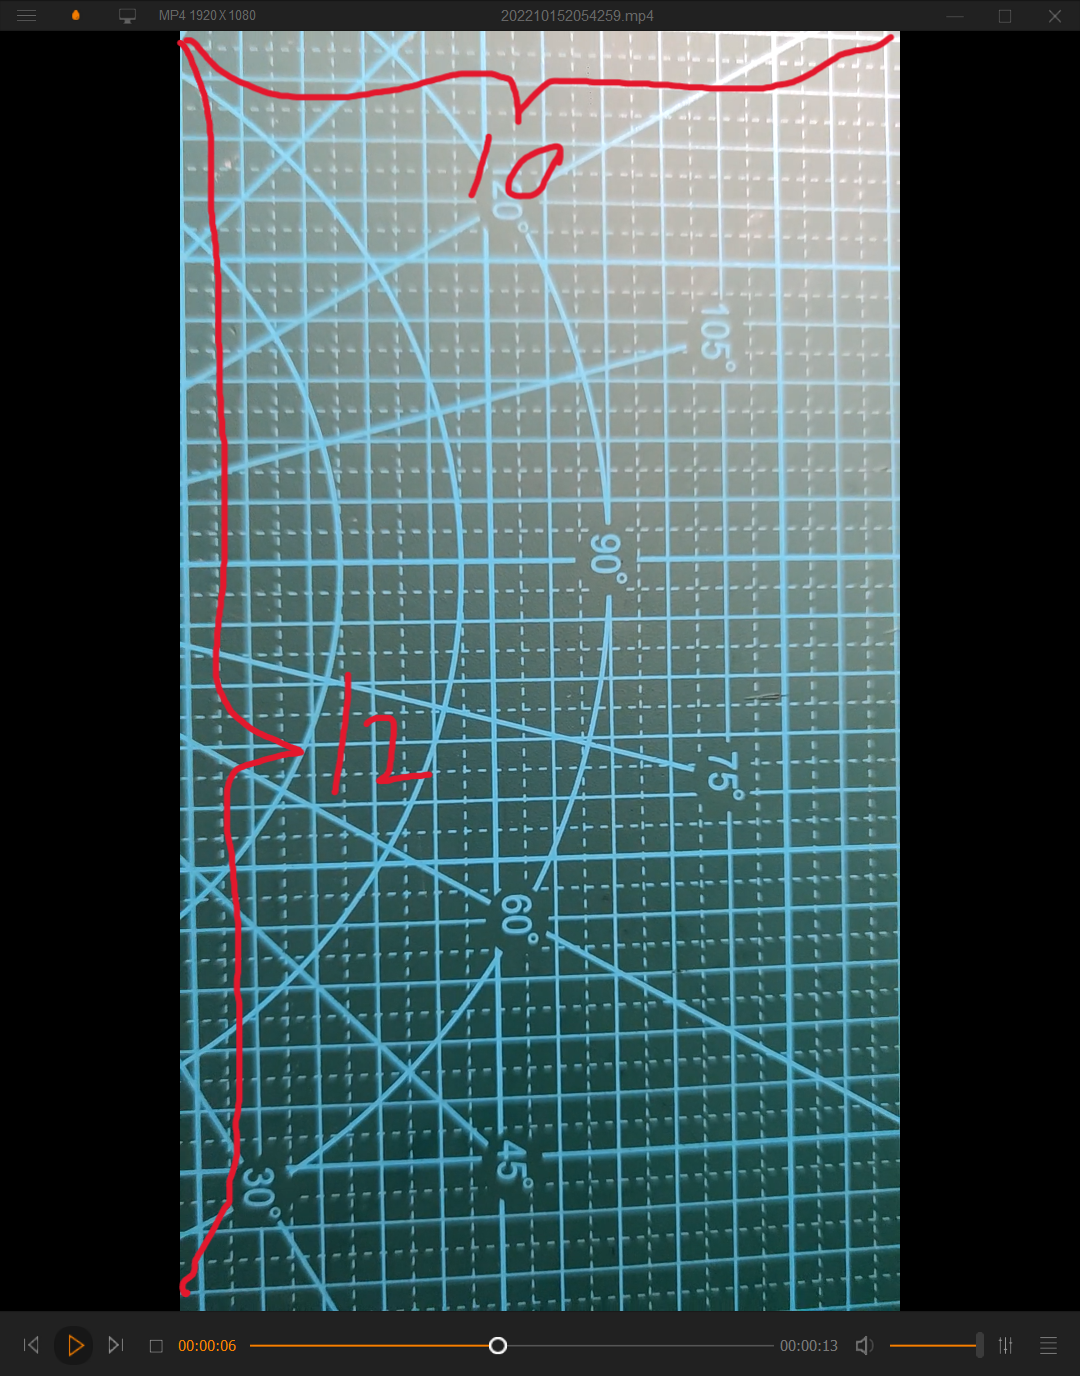
\includegraphics[height=3 in]{../pic/blocks.png}}
	\caption{Vertically Distance Estimation}
	\label{fig:blocksAndPyramid}
\end{figure}

\subsubsection{Selection of Sampling Points}

About the sampling rate (sample with my eyes), I was going to sample every 10 frames (1/6 second for a $60$ fps video), but there are so many digits for me to write down and that makes me give up. In turn, I try to decrease the points I need to write down by the way of judging the value of the points. If the point is important, like the corner, I will keep it, otherwise, I ignore it. In a word, I was trying my best to keep the shape of the trajectory and decrease the points I need to write down.

Consider things above, I draw the trajectory with python, see Fig.~\ref{fig:trajectoryOfMyPhone}.

\begin{figure}[!h]
	\centering
	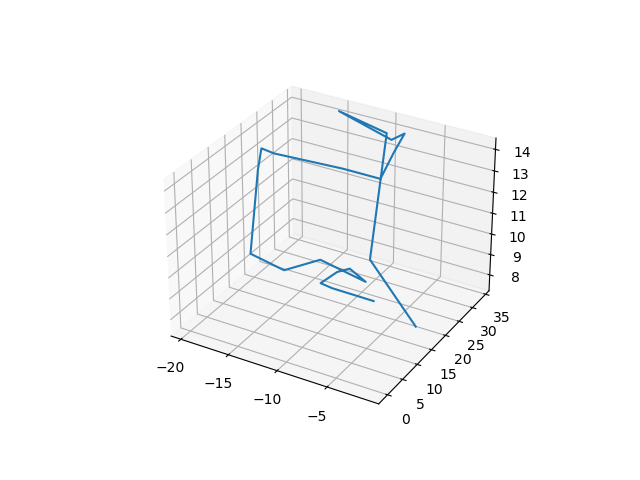
\includegraphics[width=4 in]{../pic/trajectoryOfMyPhone.png}
	\caption{Trajectory of My Phone}
	\label{fig:trajectoryOfMyPhone}
\end{figure}

\subsection{Error Analysis}
\subsubsection{Horizontal}
For the $x$ and $y$, I record the data by the format like \verb|an integer + quarters |, so the error will be within $0.5 ~ \mathrm{cm}$.
\subsubsection{Vertical}
For the $y$, the raw data is the number of blocks. The error will be about $10$ blocks, and convert to hu is $3.16 ~ \mathrm{hu}$, and convert to cm is $2.686~ \mathrm{cm}$

\section{Conclusion}
\subsubsection*{Videos}
The speed of my mouse is $16.6 ~\mathrm{m/s}$ in my calculation and $10.2 ~\mathrm{m/s}$ in official document.
\subsubsection*{Pros and Cons of Shannon/Nyquist sampling method}
Shannon/Nyquist sampling method is so ideal that it is easy to learn but hard to realize.
\subsubsection*{Trajectory of My Phone}
The trajectory is not so smooth because I don't sample enough, but it is roughly correct. The error of $x, y, z$ are all beneath a few centimeters.
\bibliographystyle{ieeetr}
\bibliography{../bib/database}

\begin{appendices}
\section{Code Listing}
\begin{python}
#plot the trajectory
from matplotlib import pyplot as plt
import numpy as np

inc = [(-1.3, -0.4, 180),
(-4, 0.1, 180),
(-1.25, 0.4, 180),
(0.3, 4.25, 180),
(-0.75, 6.5, 156),
(1, 2, 135),
(-4.75, 0.5, 144),
(-2.45, -4, 135),
(-6.5, 8.75, 104),
(1, 0, 228),
(0.25, 0.5, 264),
(1.5, -0.5, 264),
(7, 0, 270),
(3.75, 0, 270),
(-2.25, 12.25, 252),
(0.5, 2, 280),
(-1.25, -0.25, 264),
(-5.75, 1, 286),
(4.75, 0.75, 264),
(-1, -2, 84),
(8.5, -12.75, 75)]

point = [0, 0, 0]
x = []
y = []
z = []

for p in inc:
    point[0] = point[0] + p[0]
    point[1] = point[1] + p[1]
    point[2] = np.sqrt(p[2]) * 0.85
    x.append(point[0])
    y.append(point[1])
    z.append(point[2])

plt.figure()
ax = plt.axes(projection='3d')
ax.plot(x, y, z)
plt.show()
\end{python}
\begin{python}
#plot the triangular pyramid
import numpy as np
from matplotlib import pyplot as plt

x = [0, 1, 0.5, 0.5]
xx = [0.5, 0.25, 0.75, 0.5]
y = [0, 0, 0.7, 0.35]
yy = [0.35, 0.175, 0.175, 0.525]
z = [0, 0, 0, 0.6]
zz = [0.6, 0.3, 0.3, 0.3]

plt.figure()
ax = plt.axes(projection = '3d')

for i in range(4):
    for j in range(4):
        ax.scatter((x[i]),(y[i]),(z[i]),color='r')
        ax.plot((x[i],x[j]),(y[i],y[j]),(z[i],z[j]),color='b', linewidth=1)
for i in range(4):
    for j in range(4):
        ax.scatter((xx[i]),(yy[i]),(zz[i]),color='r')
        ax.plot((xx[i],xx[j]),(yy[i],yy[j]),(zz[i],zz[j]),color='b',linewidth=1)
ax.scatter(0.5, 0.35, 0,color='r')
ax.scatter(0.5, 0.35, 0.3, color='r')
ax.plot((0.5,0.5,0.5),(0.35,0.35,0.35),(0,0.3,0.6))

plt.show()
\end{python}

\end{appendices}

\end{document}